% !TeX spellcheck = de_DE
\chapter{Einleitung}
Einleitung
Motivation
Referenz auf führere IDPs (Quellen!)
didaktisches Konzept, kurz
Aufbau der Dokumentation, inkl. Benennung wer hat was gemacht (Benotung)

% Keine Beschreibung der Algorithmen an sich!

\chapter{Aufbau der Webanwendungen}
Jede Applikation ist in mehreren Teile aufgeteilt. Die Struktur von jeder Applikation ist gleich. Alle Anwendungen bestehen aus mehreren Tabs, von denen jeder eine bestimmte Fuktion hat (vgl. Abbildung~\ref{fig:tabs}).

\begin{figure}[h!]
	\centering
	
\includegraphics[width=\textwidth]{figures/tabs}
	\caption[Tabs]{Tabs der Anwendung}\label{fig:tabs}
\end{figure}

Die Tabs ``Einführung'', ``Beschreibung des Algorithmus'' und ``Weiteres'' enthalten nur den statischen Text mit Bildern und sind deswegen nicht interaktiv. Alle weiteren Tabs bieten dem Nutzer die Eingabemöglichkeiten um die Funktionen der Algorithmen zu erläutern oder seine Kentnisse zu prüfen. 

\section{Aufbau der Tabs(Aleksejs)}
\textbf{Einführung:} das Ziel des Tabs ist, eine allgemeine Vorstellung über die Anwendung dem Nutzer zu geben. Der statische Text in diesem Tab enthält einige relevante Informationen zum Problem für jeweiligen Algorithmus, ein diesem Problem entsprechendes Bild sowie zwei Tasten, die zur Erstellung des Graphs und zur Beschreibung des Algorithmus führen. Außer diesen zwei Tasten ist der Tab mit keiner weiteren Interaktivität ausgestattet.


\noindent\textbf{Graph erstellen:} in diesem Tab kann der Nutzer einen Graph erstellen, auf dem der Algorithmus später ausgeführt wird. Hier stehen zwei Möglichkeiten zur Verfügung: entweder den Graph selbst mit der Maus zu erstellen oder einen fertigen Graph aus der vorgegebenen Liste zu wählen. Falls der Algorithmus einen gewichteten Graph voraussetzt, kann der Nutzer die Gewichte nach dem Doppelklick auf der Kante selbst eingeben. Wenn der Algorithmus einen bipartiten Graph erfordert, dann wird die Erstellung des Graph beschränkt, damit alle Eigenschaften des bipartiten Graphs erfüllt sind. 

\noindent\textbf{Algorithmus ausführen:} hier wird der Ablauf des Algorithmus dargestellt. Der Algorithmus läuft auf dem Graph, der im vorigen Tab erstellt wurde. Man kann sowohl schrittweise den Algorithmus ausführen als auch den vorspulen. Außerdem kann der Nutzer den Schnellvorlauf pausieren, in diesem Fall wird der Ablauf im aktuellen Schritt gestoppt. Bei jedem Schritt wird die entsprechende Information zum Status des Algorithmus aufgezeigt und der Stand des Pseudocodes wird im separaten Fenster abgebildet.

\noindent\textbf{Beschreibung des Algorithmus:} dieser Tab stellt die ausführliche Informationen zum jeweiligen Algorithmus dar. Der Tab enthält statischen Text mit Bildern, der die Logik des Algorithmus erklärt. Im unteren Teil des Tabs stehen die Tasten, die auf anderen Tabs verweisen.

\noindent\textbf{Forschungsaufgaben:} bei jeder Anwendung stehen zwei Tabs zur Verfügung, wo der Nutzer die Aufgaben lösen muss. Der Zweck der Forschungsaufgaben ist zu prüfen, wie gut der Nutzer die Algorithmen verstanden hat. In den Aufgaben wird gefragt, welche Entscheidungen der Algorithmus trifft. Am Ende der Aufgabe sieht man die Statistik, die die Antworten des Nutzers erfasst. Danach wird vorgeschlagen zu weiteren Tabs der Applikation zu gehen.

\noindent\textbf{Weiteres:} im letzten Tab kann der Nutzer weitere Informationen zum Algorithmus lesen. Es handelt sich um den Pseudocode, die Laufzeit der Algorithmen, den Beweis der Korrektheit und die Links zu sonstigen Quellen.

\section{Algorithmus von Floyd-Warshall(Aleksejs)}
Da die Implementierung des Floyd-Warshall Algorithmus nicht kompliziert ist, war es wichtig zu zeigen, was genau während dem Ablauf schrittweise passiert. Der Algorithmus wurde in Schritte so unterteilt, dass jeder Schritt eine Verbesserung der Distanz zwischen zwei Knoten darstellt. Um die Verbesserungen anschaulich zu machen, wurde die Adjazenzmatrix implementiert. In jeder Zelle der Adjazenzmatrix wird der aktuelle Distanzwert zwischen zwei entsprechenden Knoten gespeichert. Wenn man die Maus über eine Zelle in der Matrix bewegt, dann wird der Pfad, der diesem Distanzwert entspricht, im Graphen markiert (vgl. Abbildung~\ref{fig:fw-matrix}).

\begin{figure}[h!]
	\centering
	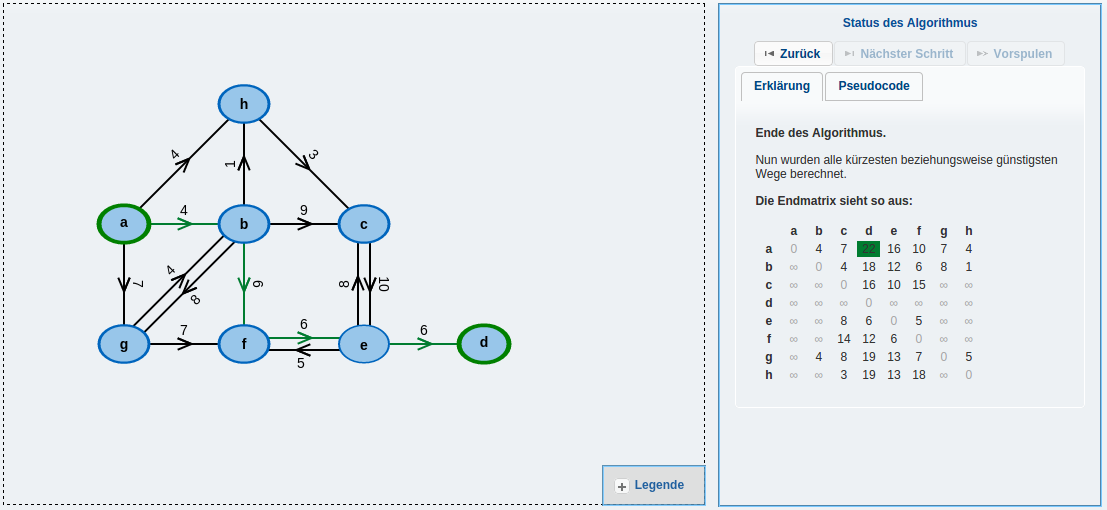
\includegraphics[width=\textwidth]{figures/fw-matrix}
	\caption[Floyd-Warshall Matrix]{Visualisierung des verbesserten Pfades}\label{fig:fw-matrix}
\end{figure}

Die erste Forschungsaufgabe prüft, ob der Nutzer die Logik des Algorithmus verstanden hat. Während des Ablaufs von Floyd-Warshall auf dem bestimmten Graphen werden die Fragen über die vom Algorithmus getroffenen Entscheidungen gestellt.

In der zweiten Forschungsaufgabe soll der Nutzer die fehlende Kantengewichte bestimmen. Ein Teil der Kantenkosten sowie die Adjazenzmatrix sind am Anfang gegeben. Diese Information muss genutzt werden um die fehlende Gewichte zu bestimmen.

\section{Algorithmus von Hierholzer (Mark)}
Beim Algorithmus von Hierholzer war es uns wichtig, die resultierende Eulertour verständlich zu visualisieren. Dazu werden zunächst alle Subtouren in unterschiedlichen Farben dargestellt. Einzelne Subtouren können auf der Ergebnisseite einzeln hervorgehoben werden. Der Benutzer erkennt mittels der Farben außerdem, welcher Teil der Tour aus welcher Subtour stammt. Die Tour kann durch eine Animation (vgl. Abbildung~\ref{fig:hierholzer-animation}) in der richtigen Reihenfolge abgelaufen werden, sodass der Nutzer verifizieren kann, dass es sich wirklich um eine Eulertour handelt.

\begin{figure}[h!]
	\centering
	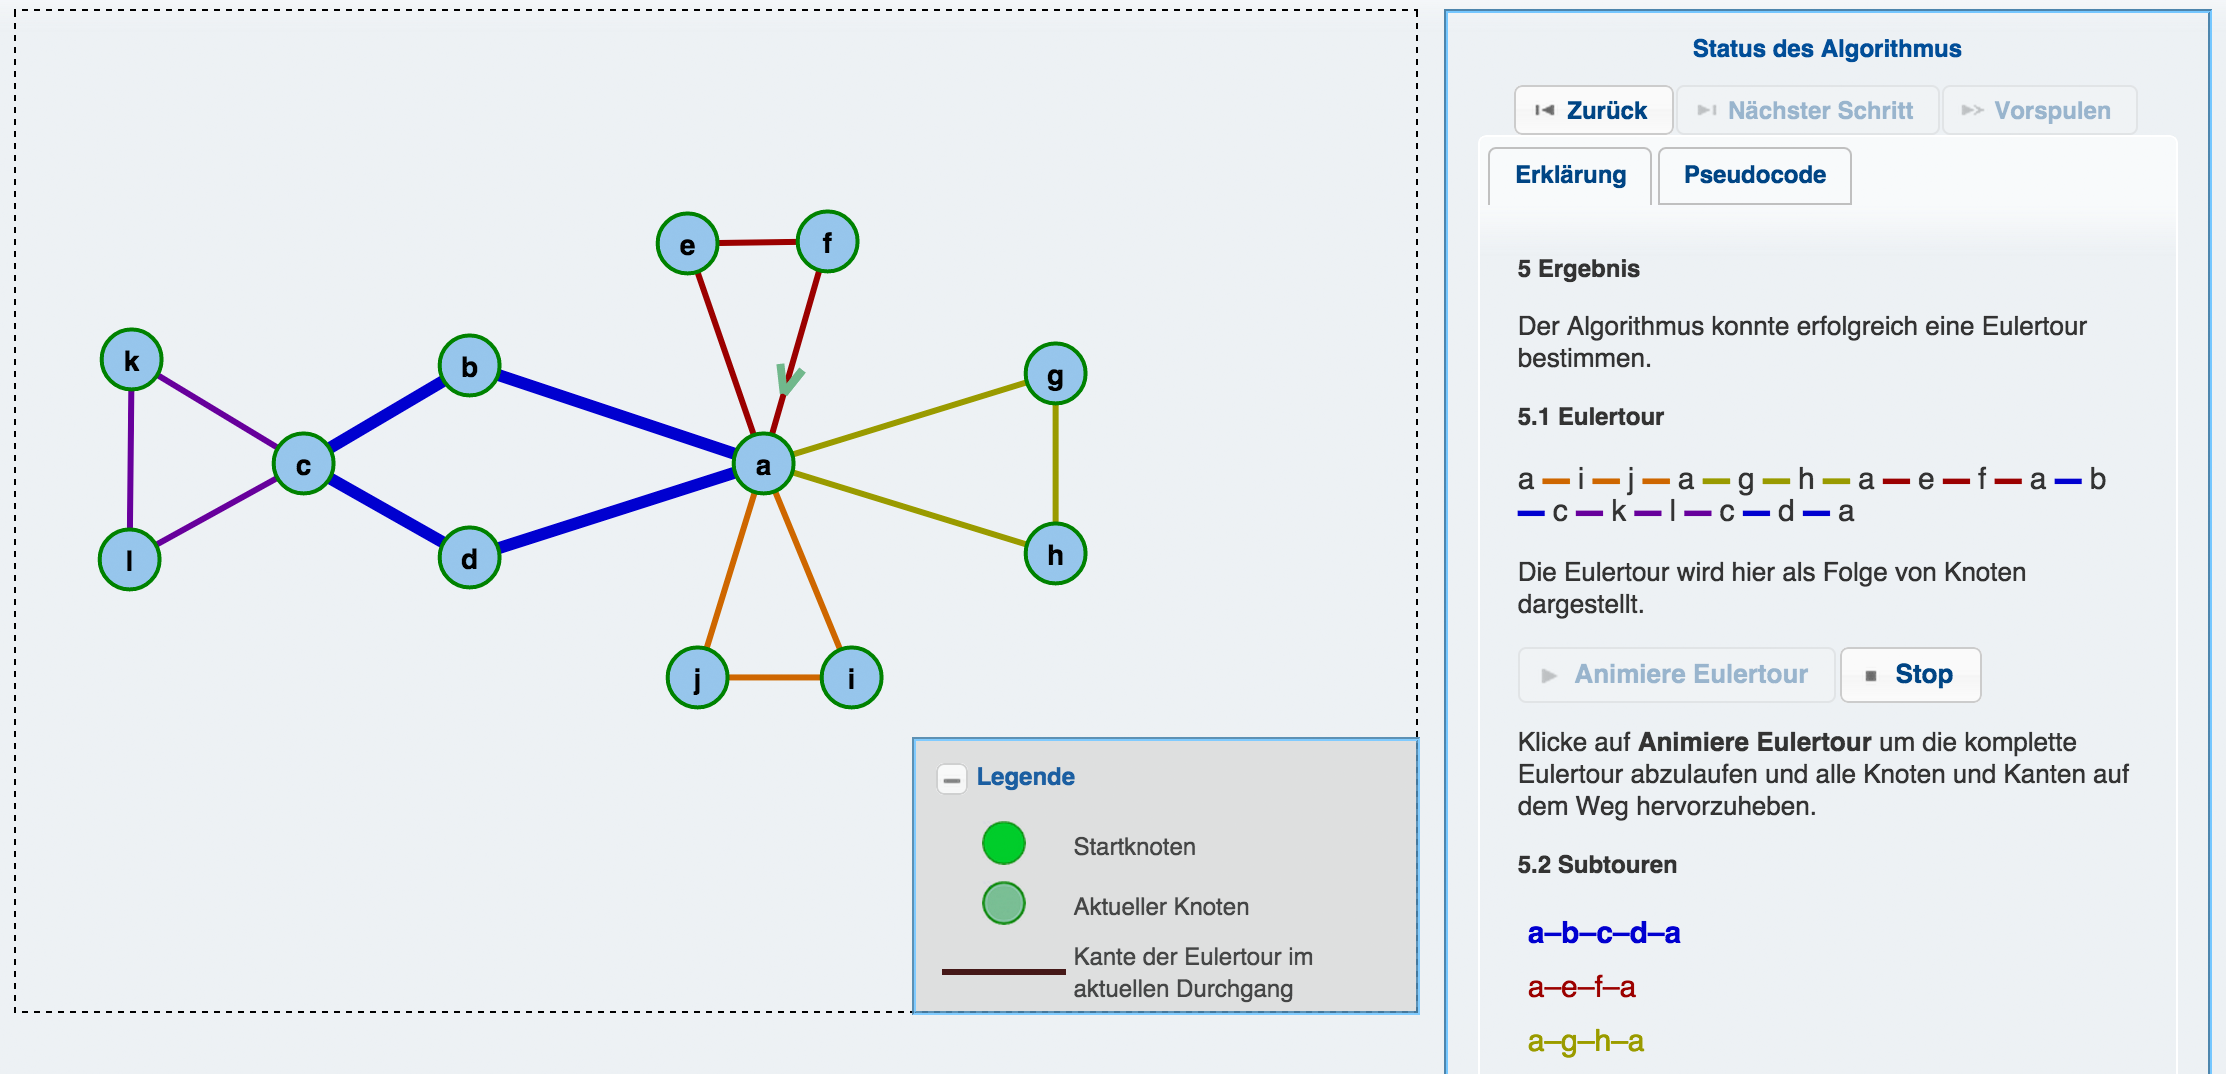
\includegraphics[width=\textwidth]{figures/hierholzer_animation}
	\caption[Eulertour Animation]{Visualisierung der Eulertour mittels Animation}\label{fig:hierholzer-animation}
\end{figure}

Die erste Forschungsaufgabe soll sicherstellen, dass der Nutzer die wichtigsten Abläufe des Algorithmus versteht. Sie behandelt daher im Wesentlichen den Ablauf des Algorithmus, das Konzept des Knotengrads und das Verbinden von Touren.

In einer weiteren Forschungsaufgabe werden die Besonderheiten des Algorithmus bei Anwendung auf einen gerichteten Graphen betrachtet. Der Nutzer betrachtet die geänderten Voraussetzungen, die der Graph erfüllen muss und die veränderte Auswahl der Kanten zur Konstruktion von Subtouren.
     
\section{Algorithmus von Hopcroft und Karp}%Ruslan
Der Algorithmus wurde in Phasen unterteilt. In jeder Phase des Algorithmen wird nach einer inklusions-maximalen Menge von kürzesten disjunkten Augmentationswegen gesucht. Die in einer Phase gefundenen Augmentationswege werden nacheinander hervorgehoben und das Matching augmentiert.
Das Aufzeigen der Augmentationswege stand im Fokus bei der Visualisierung des Algorithmen. Der Benutzter sollte diese leicht erkennen und nachvollziehen können. Um das Konzept von disjunkten Augmentationswegen zu verdeutlichen, werden die Knoten der bereits verarbeiteten Augmentationswegen grau markiert. Dadurch wird dem Benutzer verdeutlicht, dass ein Knoten in einer Phase nur auf einem Augmentationsweg vorkommt. 
Die graue Markierung der benutzten Knoten sollte außerdem hervorheben, dass die Menge von disjunkten Augmentationswegen inklusions-maximal ist. Der Benutzer kann am Ende einer Phase leicht nachvollziehen, dass es keinen weiteren disjunkten kürzesten Augmentationsweg existiert.

\begin{figure}[h!]
	\centering
	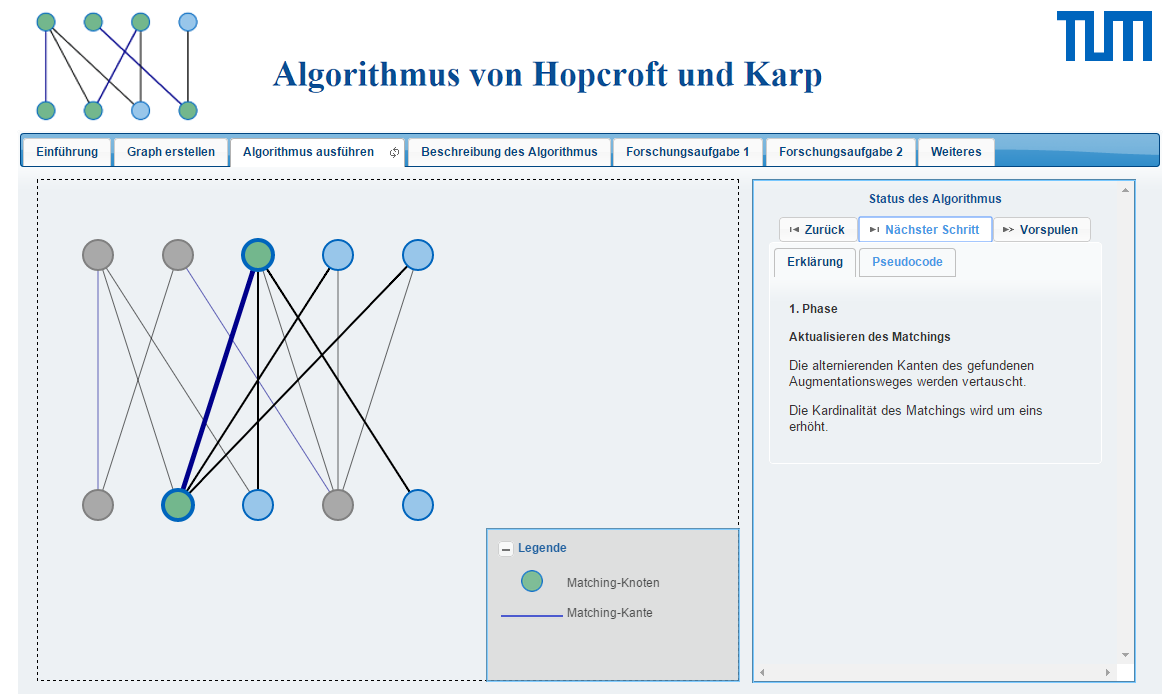
\includegraphics[width=\textwidth]{figures/hopcroft_karp_augmentation}
	\caption[Augmentationsweg]{Hervorhebung des aktuellen Augmentationsweges im Hopcroft-Karp-Algorithmus}\label{fig:hopcroft_karp_augmentation}
\end{figure}

In der ersten Forschungsaufgabe soll der Nutzer sein Verständnis über den Ablauf des Algorithmen prüfen. Der Benutzer sollte das Konzept von kürzesten Augmentationswegen verstehen und wissen, welche Kanten nach einem Augmentationsschritt im Matching sein werden.

In der zweiten Forschungsaufgabe bekommt der Nutzer die Gelegenheit mit Augmentationswegen zu experimentieren. Der Algorithmus stoppt zufällig an einigen Stellen, wo der Benutzer einen Augmentationsweg selbst einzeichnen soll. Es müssen nicht die kürzesten Augmentationswege eingezeichnet werden. Der Benutzer sollte sehen, wie seine Wahl die weitere Ausführung des Algorithmen beeinflusst.

\section{Ungarische Methode(Aleksejs)}
Obwohl es mehrere Implementierungen der Ungarischen Methode gibt, die Idee bleibt bei allen gleich. Die Applikation geht nicht tief in die Einzelheiten der konkreten Implementierung, sondern erklärt das generelle Prinzip der Ungarischen Methode. Dafür war der Einsatz des bipartiten gewichteten Graphs notwendig. Als die Ungarische Methode perfektes Matching im bipartiten Graphen sucht, wird eingegebener Graph in der Anwendung bis zum kompletten Graphen vervollständigt falls der Nutzer das nicht gemacht hat. Um die genutzte Begriffe (wie z. B. Matching oder Augmentationsweg) verständlich zu machen, werden unterschiedliche Farben für Knoten und Kanten während des Ablaufs verwendet (vgl. Abbildung~\ref{fig:hungarian-colors}).
\begin{figure}[h!]
	\centering
	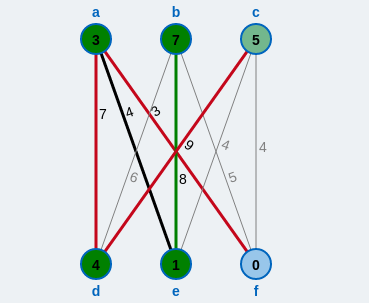
\includegraphics[width=\textwidth]{figures/hungarian-colors}
	\caption[Ungarische Methode]{Augmentationsweg wird rot markiert}\label{fig:hungarian-colors}
\end{figure}

Die erste Forschungsaufgabe prüft, wie gut der Nutzer den Aufbau des Algorithmus verstanden hat. Dazu werden die Fragen während des Ablaufs auf dem beliebigen Graphen gestellt. Der Nutzer muss beantworten, wie der Algorithmus die Markierungen zuweist und welche Schritte macht der Algorithmus als weitere. 

Bei der zweiten Forschungsaufgabe werden auch die Fragen während des Ablaufs der Ungarischen Methode gestellt. Der Graph ist in diesem Fall bestimmt und die Fragen fassen den Aufbau des Augmentationsweges und Gleichheitsgraphs um.

\section{Chinese-Postman-Algorithmus}%Ruslan
%Besonderes
Der implementierte Chinese-Postman-Algorithmus löst das gerichtete Chinese-Postman-Problem. 
Das Besondere bei dem Chinese-Postman-Algorithmus ist, dass er für die Ausführung weitere Algorithmen benötigt. Diese sind 
\begin{itemize}
\item Floyd-Warshall-Algorithmus
\item Ungarische Methode
\item Hierholzer-Algorithmus
\end{itemize}
Der Algorithmus ist in verschiedene Schritte eingeteilt. Zuerst wird überprüft, ob das Problem auf dem Graphen lösbar ist. Anschließend wird eine Menge von Pfaden gesucht, sodass nach dem Einfügen dieser Pfade in den Graphen der Graph eulersch wird. Die Summe der Längen dieser Pfade sollte minimal sein.
Zum Schluss wird ein Eulerkreis im Graphen gefunden, was die Lösung des Problems darstellt.

%Visualisierung
Um die optimale Menge von zusätzlichen Pfaden zu bestimmen, werden zuerst Knoten bestimmt, bei denen die Anzahl der Eingangs- und Ausgangskanten nicht übereinstimmt.
Abhängig davon, ob es zu viele Eingangs- oder Ausgangsknoten gibt, werden diese Knoten hell- bzw. dunkelfarbig markiert(vgl. Abbildung~\ref{fig:unbalanced}). Außerdem wird die Differenz zwischen Ausgangs- und Eingangsgrad eines Knoten im Knoten gezeigt. Dadurch entstehen zwei Partitionen von Knoten. 
%Der Nutzer sieht damit sofort, zwischen welchen Knoten neue Pfade eingefügt werden müssen.

\begin{figure}[h!]
	\centering
	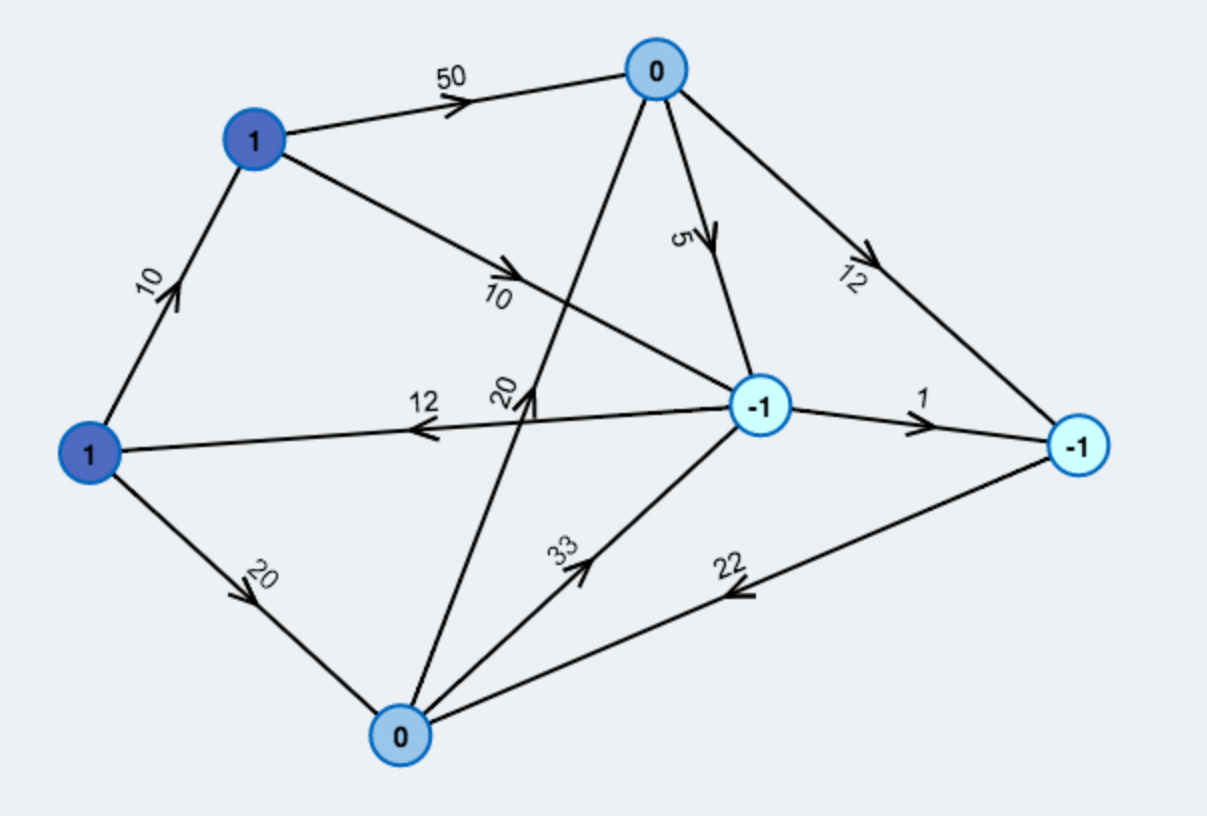
\includegraphics[width=0.8\textwidth]{figures/postman_unbalanced}
	\caption[Unbalancierte Knoten]{Hervorheben von Knoten mit ungleichem Eingangs- und Ausgangsgrad}\label{fig:postman_unbalanced}
\end{figure}

Im nächsten Schritt wird ein bipartiter Graph erstellt, der aus den markierten Knoten besteht. Um den Wechsel von dem Ausgangsgraphen zu dem bipartiten Graphen nachvollziehbar zu gestalten, wurde eine Animation eingefügt. Alle für den Matching-Graphen relevanten Knoten werden aus dem Graphen herausgenommen und zu dem bipartiten Matching-Graphen transportiert. Das Aussehen des Matching-Graphen wurde aus der Ungarischen Methode übernommen. 

\begin{figure}[h!]
	\centering
	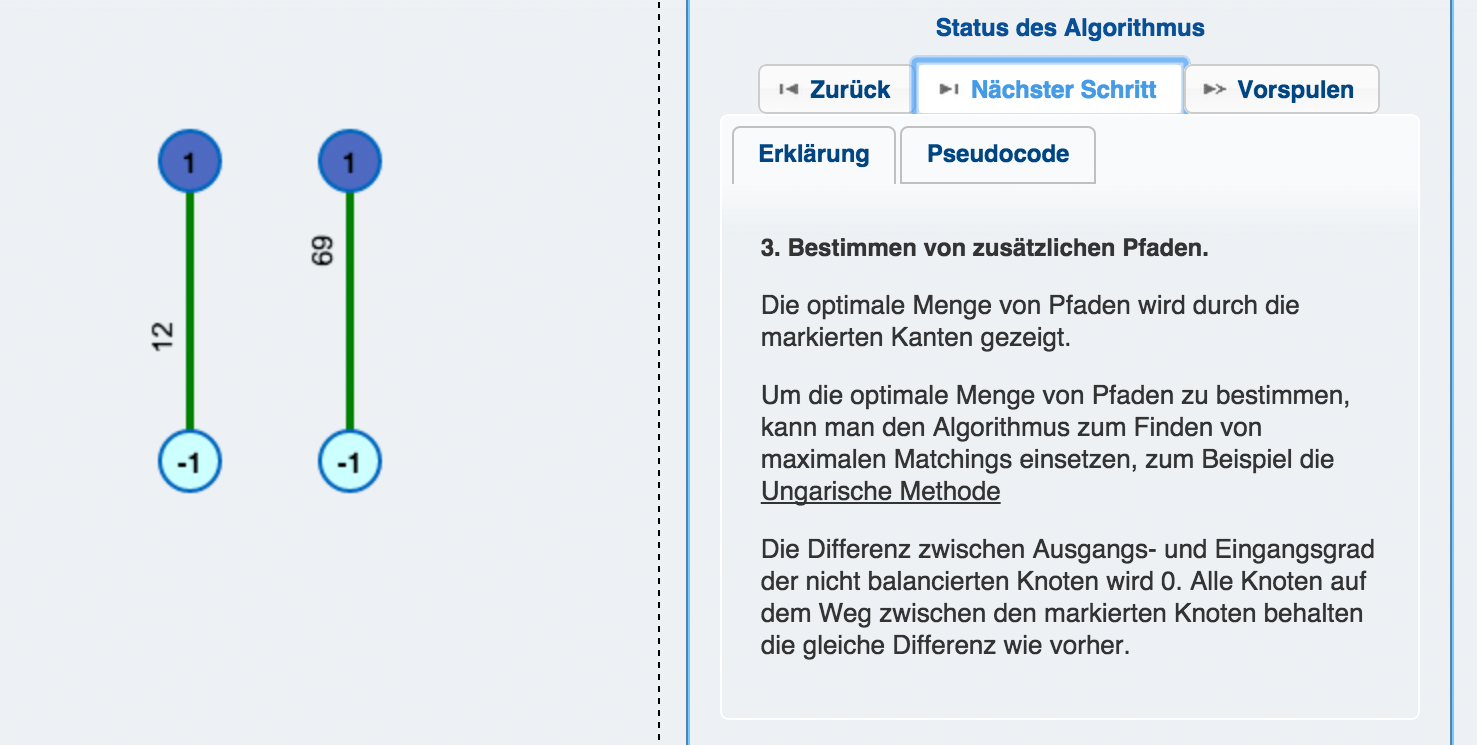
\includegraphics[]{figures/postman_matching}
	\caption[Matching]{Matchinggraph }\label{fig:postman_matching}
\end{figure}

In der Implementierung des Algorithmen bestimmt die Differenz zwischen Ausgangs- und Eingangsgrad eines Knotens, wie oft dieser im Matching-Graphen vorkommt. Es entsteht ein vollständiger bipartiter Graph, sodass mit der Ungarischen-Methode-Algorithmus ein optimales Matching bestimmt werden kann. Das Gewicht einer Kante ist die Länge des kürzesten Weges von dem Knoten mit negativer Differenz zwischen Ausgangs- und Eingangsgrad zu dem Knoten mit positiver Differenz. Bei der Visualisierung des Algorithmen wurde eine Entscheidung zugunsten Übersichtlichkeit getroffen, sodass ein Knoten nur einmal im Matching-Graphen vorkommen sollte. Dadurch wird für den Nutzer nachvollziehbar, zwischen welchen Knoten neue Wege eingefügt werden müssen. Die Differenz zwischen Ausgangs- und Eingangsgrad eines Knotens bestimmt die Anzahl von Pfaden, die in diesem Knoten enden bzw. anfangen müssen und somit die Anzahl von Matching-Kanten, die zu diesem Knoten inzident sind.

Nachdem die optimalen Pfade im Matching-Schritt bestimmt wurden, werden die Knoten wieder an ihren Platz in den normalen Graphen transportiert. Allerdings werden die Matching-Kanten ebenfalls in den Graphen übernommen. Der Benutzer sieht somit auch im normalen Graphen, zwischen welchen Knoten neue Wege eingefügt werden müssen.
Das Einfügen von neuen Pfaden wird ebenfalls mittels einer Animation aufgezeigt. Die aktuelle Matching-Kante wird markiert und die Kanten auf dem neuen Weg werden schrittweise in den Graphen eingefügt. Anschießend wird die Matching-Kante gelöscht.

Am Ende des Algorithmen wird die Eulertour des Graphen bestimmt. Der Nutzer kann die Animation der Tour selbst starten und stoppen. Die Visualisierung der Eulertour ist aus dem Hierholzer-Algorithmus übernommen.

\begin{figure}[h!]
	\centering
	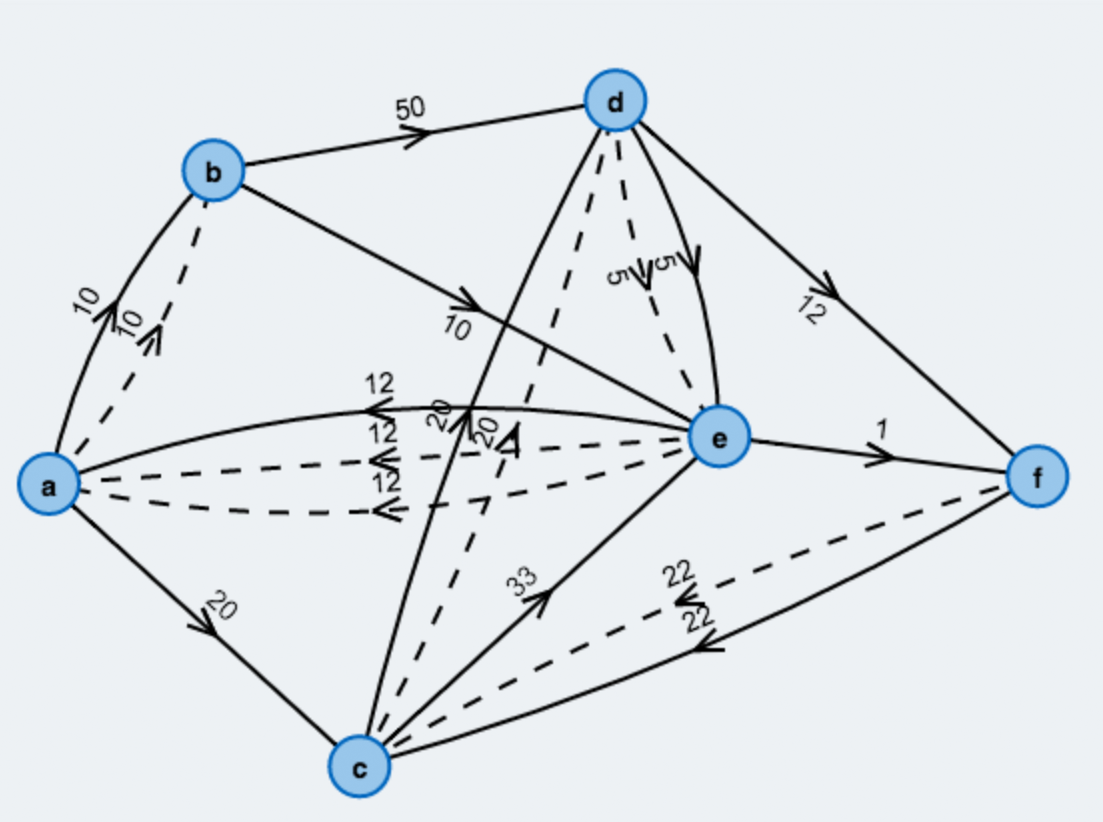
\includegraphics[width=0.8\textwidth]{figures/postman_eulerian}
	\caption[Eulerscher Graph]{Graph nach Einfügen von zusätzlichen Pfaden}\label{fig:postman_eulerian}
\end{figure}

%Forschungsaufgaben
Die erste Forschungsaufgabe sollte das Wissen des Benutzers prüfen. Der Benutzer sollte verstehen, welche Knoten im Matching-Graphen gebraucht werden und wie viele zusätzliche Wege in einem Knoten starten bzw. enden müssen.

Die zweite Forschungsaufgabe lässt dem Benutzer die Möglichkeit den Rundweg selbst zu bestimmen, der alle Kanten des Graphen enthält. Anschließend wird die Länge dieses Weges mit der optimalen Lösung verglichen. Der Benutzer kann dadurch feststellen, inwiefern seine Lösung von der optimalen Lösung abweicht.

\chapter{Implementierung}

\section{Installation (Mark)}
Zur Installation sind keine speziellen Anforderungen zu erfüllen. Die Webapplikationen wurden vollständig mittels HTML5, JavaScript und CSS implementiert, sodass keine zusätzliche serverseitige Software benötigt wird. Zum Aufrufen der Anwendungen wird ein moderner Webbrowser benötigt.

Die Bereitstellung erfolgt über den Online Dienst GitHub, der das verteile Versionskontrollsystem Git benutzt. 
Alle Anwendungen liegen in einem gemeinsamen Repository, welches unter \url{https://github.com/herzog31/adv-graph-algorithms} erreichbar ist. Zur Installation kann man entweder auf der Repository Seite die letzte freigegebene Version (Release) als Zip oder Tar Archiv herunterladen oder die aktuellste Version des Repositories mittels folgendem Befehl in das aktuelle Verzeichnis kopieren.

\begin{figure}[h!]
\begin{lstlisting}[language=Bash]
git clone -b master https://github.com/herzog31/adv-graph-algorithms.git
\end{lstlisting}
\caption[Repository Kopieren]{Befehl zum Kopieren des GitHub Repositories}\label{fig:listing-github}
\end{figure}

Um die Anwendungen als Webanwendungen online bereitzustellen wird ein Webserver benötigt. Hier emfiehlt sich die Installation des Apache oder nginx  HTTP Servers.

Die lokale Ausführung ist ohne einen Webserver möglich. Verschiedene Webbrowser besitzen allerdings eine Sicherheitsrichtlinie, die das Öffnen von lokalen Dateien über JavaScript verbieten. Diese Sicherheitsrichtline kann jedoch durch spezielle Einstellungen umgangen werden. Für Google Chrome ist dies über den Start Parameter \texttt{--allow-file-access-from-files} möglich.

\section{MathJAX (Mark)}
Unter den Tabs \enquote{Beschreibung des Algorithmus} werden die komplizierten Algorithmen, wie bspw. die Ungarische Methode, in möglichst einfachen Worten als Fließtext erklärt. Wir gehen davon aus, dass der Nutzer während der Bearbeitung der Forschungsaufgaben, verschiedene Sachverhalte in der Algorithmenbeschreibung nachschlagen muss. Das wiederholte Lesen von vollständigen Absätzen wollten wir allerdings vermeiden.

Dazu haben wir zusätzlich zur textuellen Beschreibung, wichtige Punkte der Algorithmen auch als mathematische Formeln dargestellt. Der Nutzer erlangt so durch das erste Lesen der Beschreibung ein Grundverständnis der Algorithmen und kann während der Bearbeitung aufkommende Fragen durch die dargestellten Formeln schneller erschließen.

Zur Darstellung der Formeln in den Webapplikationen verwenden wir JavaScript Bibliothek MathJAX\footnote{https://www.mathjax.org/}. Diese ist frei unter der Apache-Lizenz erhältlich und wird u.a. auch von Wikipedia zur Darstellung jeglicher mathematischer Ausdrücke genutzt. Mit der Bibliothek ist es möglich mit LaTeX beschriebene Ausdrücke als SVG oder PNG im Webbrowser zu rendern. 

Damit die Bibliothek in den Webanwendungen genutzt werden kann, muss sie wie folgt eingebunden werden (vgl. Abbildung~\ref{fig:listing-mathjax-include}.

\begin{figure}[h!]
\begin{lstlisting}[language=HTML]
<script type="text/javascript" src="../library/js/mathjax/MathJax.js?config=TeX-AMS-MML_SVG.js&locale=de"></script>
<script type="text/x-mathjax-config">
	MathJax.Hub.Config({
		showMathMenu: false,
		showMathMenuMSIE: false
	});
</script>
\end{lstlisting}
\caption[MathJAX Einbindung]{Einbinden der MathJAX Bibliothek}\label{fig:listing-mathjax-include}
\end{figure}

Nach der Einbindung werden sämtliche LaTeX Ausdrücke welche sich zwischen den Begrenzungszeichen \texttt{\textbackslash(} und \texttt{\textbackslash)} befinden, automatisch übersetzt. In einem Beispiel wird hier der HTML Code in Abbildung~\ref{fig:listing-mathjax-example-html} von MathJAX im Browser gerendert (vgl. Abbildung~\ref{fig:mathjax-example-img}.

\begin{figure}[h!]
\begin{lstlisting}[language=HTML]
<p style="text-align: center;">
	\(\Delta = \min\limits_{s \in S\ \wedge\ y \in Y \setminus T}\{l(s) + l(y) - w(s,y)\}\)
</p>
\end{lstlisting}
\caption[MathJAX Beispiel Code]{MathJAX Beispiel: HTML Code}\label{fig:listing-mathjax-example-html}
\end{figure}

\begin{figure}[h!]
	\centering
	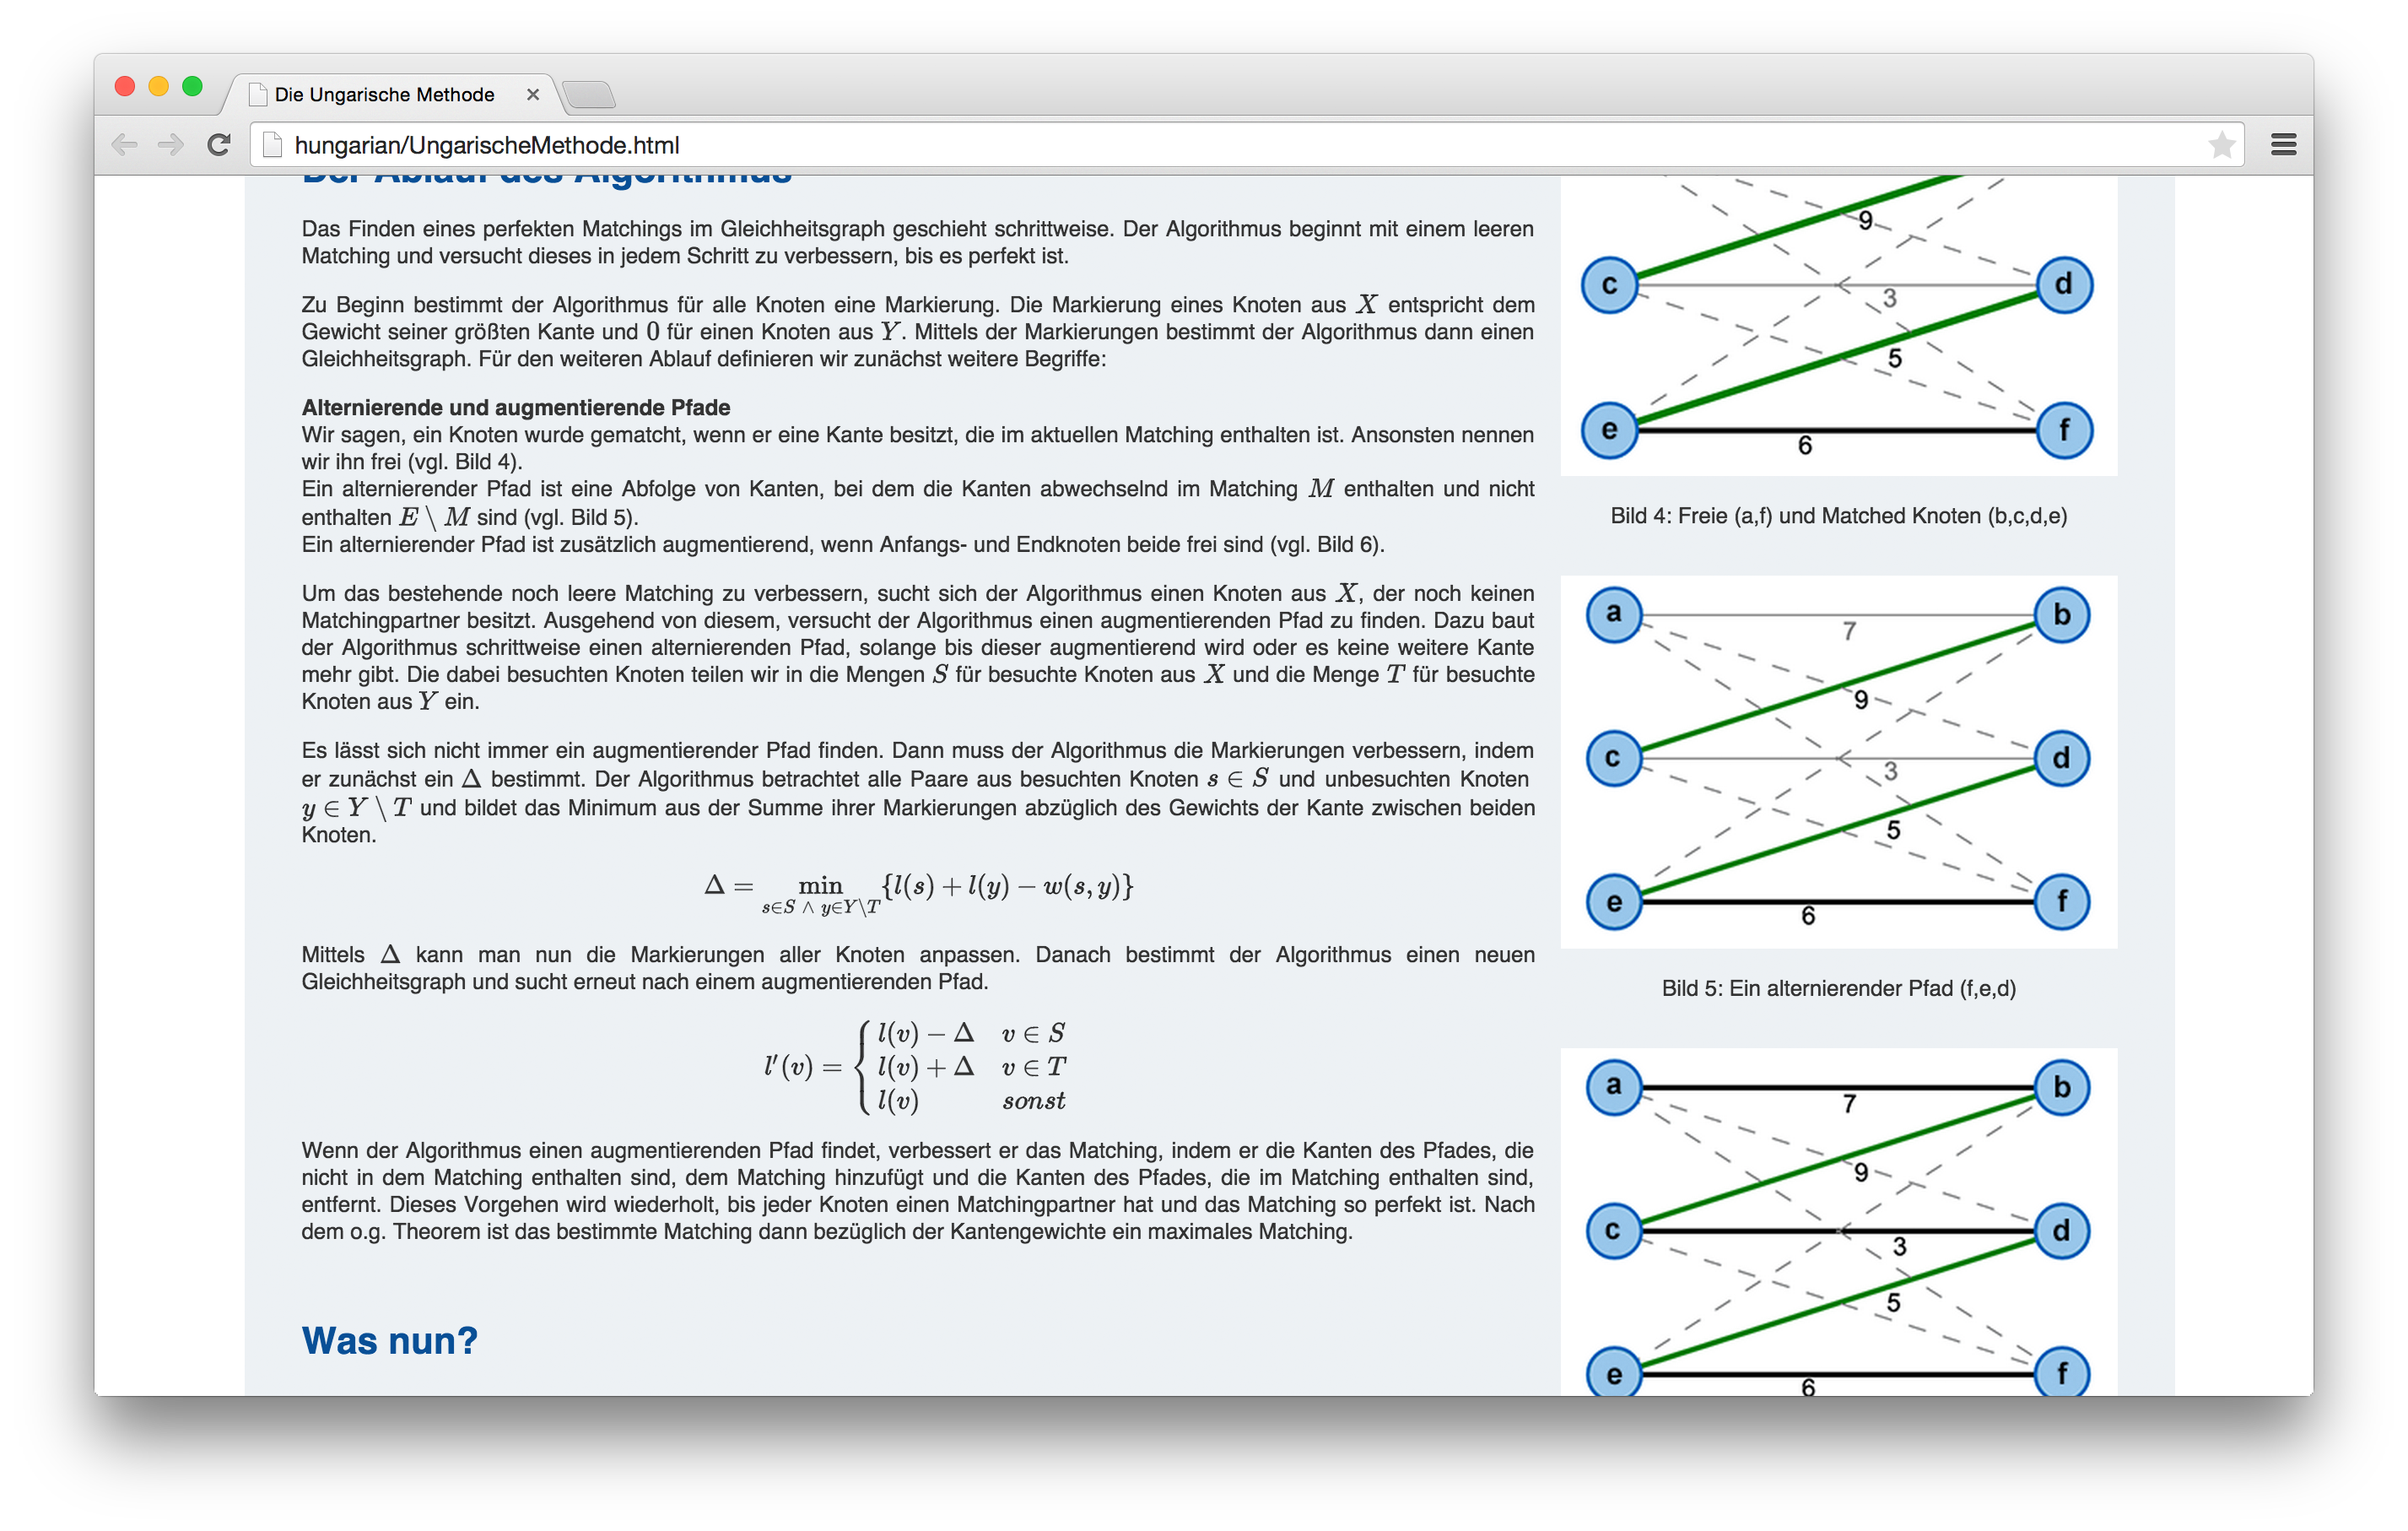
\includegraphics[width=\textwidth]{figures/mathjax-example}
	\caption[MathJAX Beispiel Browser]{MathJAX Beispiel: Darstellung im Browser}\label{fig:mathjax-example-img}
\end{figure}

Werden Ausdrücke zur Laufzeit in das DOM mittels JavaScript eingefügt, so müssen diese separat übersetzt werden (vgl. Abbildung~\ref{fig:listing-mathjax-render}).

\begin{figure}[h!]
\begin{lstlisting}[language=JavaScript]
MathJax.Hub.Queue(["Typeset", MathJax.Hub]);
\end{lstlisting}
\caption[MathJAX Render Befehl]{Befehl zum erneuten Rendern von Ausdrücken im HTML Dokument}\label{fig:listing-mathjax-render}
\end{figure}

\section{Bipartite Graphen(Aleksejs)}
Zwei Algorithmen, die im Rahmen des Projekts implementiert wurden, nämlich Hopcroft \& Karp Algorithmus und die Ungarische Methode, müssen auf bipartiten Graphen ausgeführt werden. Dafür haben wir das Konzept des bipartiten Graphen im existierenden Framework entwickelt. Um die Darstellung des Matching-Problems und dessen Lösung möglichst anschaulich zu machen, haben wir die Knoten im Graphen in zwei Gruppen geteilt (vgl. Abbildung~\ref{fig:hungarian-bipartite}). Die Kanten können nur zwischen den Knotengruppen erstellt werden. Bei der Ungarischen Methode war es wichtig den Graph mit extra Knoten und Kanten zu vervollständigen, wenn der ursprüngliche Graph nicht komplett war. Das ist notwendig, weil die Ungarische Methode perfektes Matching sucht.
\begin{figure}[h!]
	\centering
	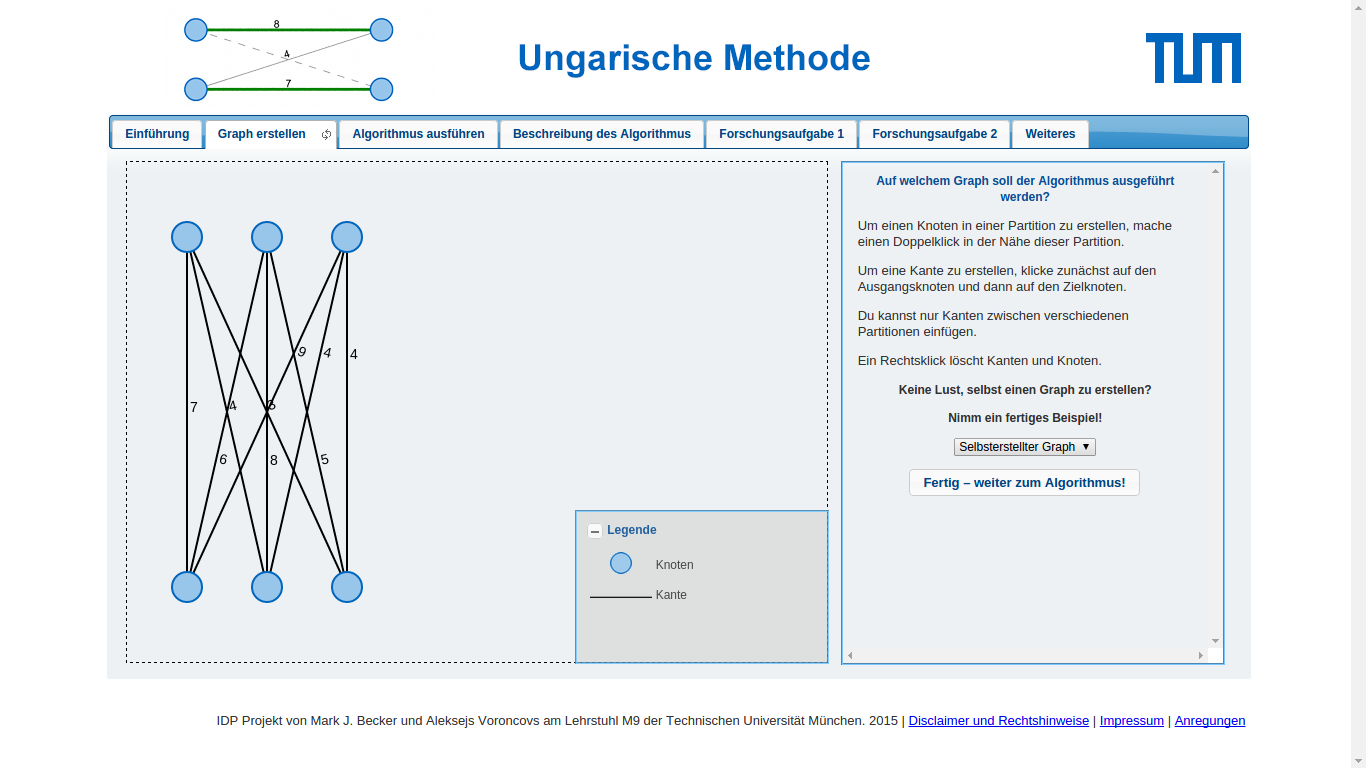
\includegraphics[width=\textwidth]{figures/hungarian-bipartite}
	\caption[Ungarische Methode]{Bipartiter Graph}\label{fig:hungarian-bipartite}
\end{figure}

In der Abbildung~\ref{fig:hungarian-complete} kann man sehen, was passiert, wenn man bei der Ungarischen Methode einen nicht kompletten Graphen eingibt. Falls eine Kante zwischen beliebigen zwei Knoten fehlt, wird eine zusätzliche graue Kante mit dem Gewicht 0 hinzugefügt. Wenn die Knotengruppen ungleiche Anzahl der Knoten enthalten, dann werden zusätzliche Knoten dem Graphen hinzugefügt. Alle Nachbarkanten bei diesen zusätzlichen Knoten haben das Gewicht 0.
\begin{figure}[h!]
	\centering
	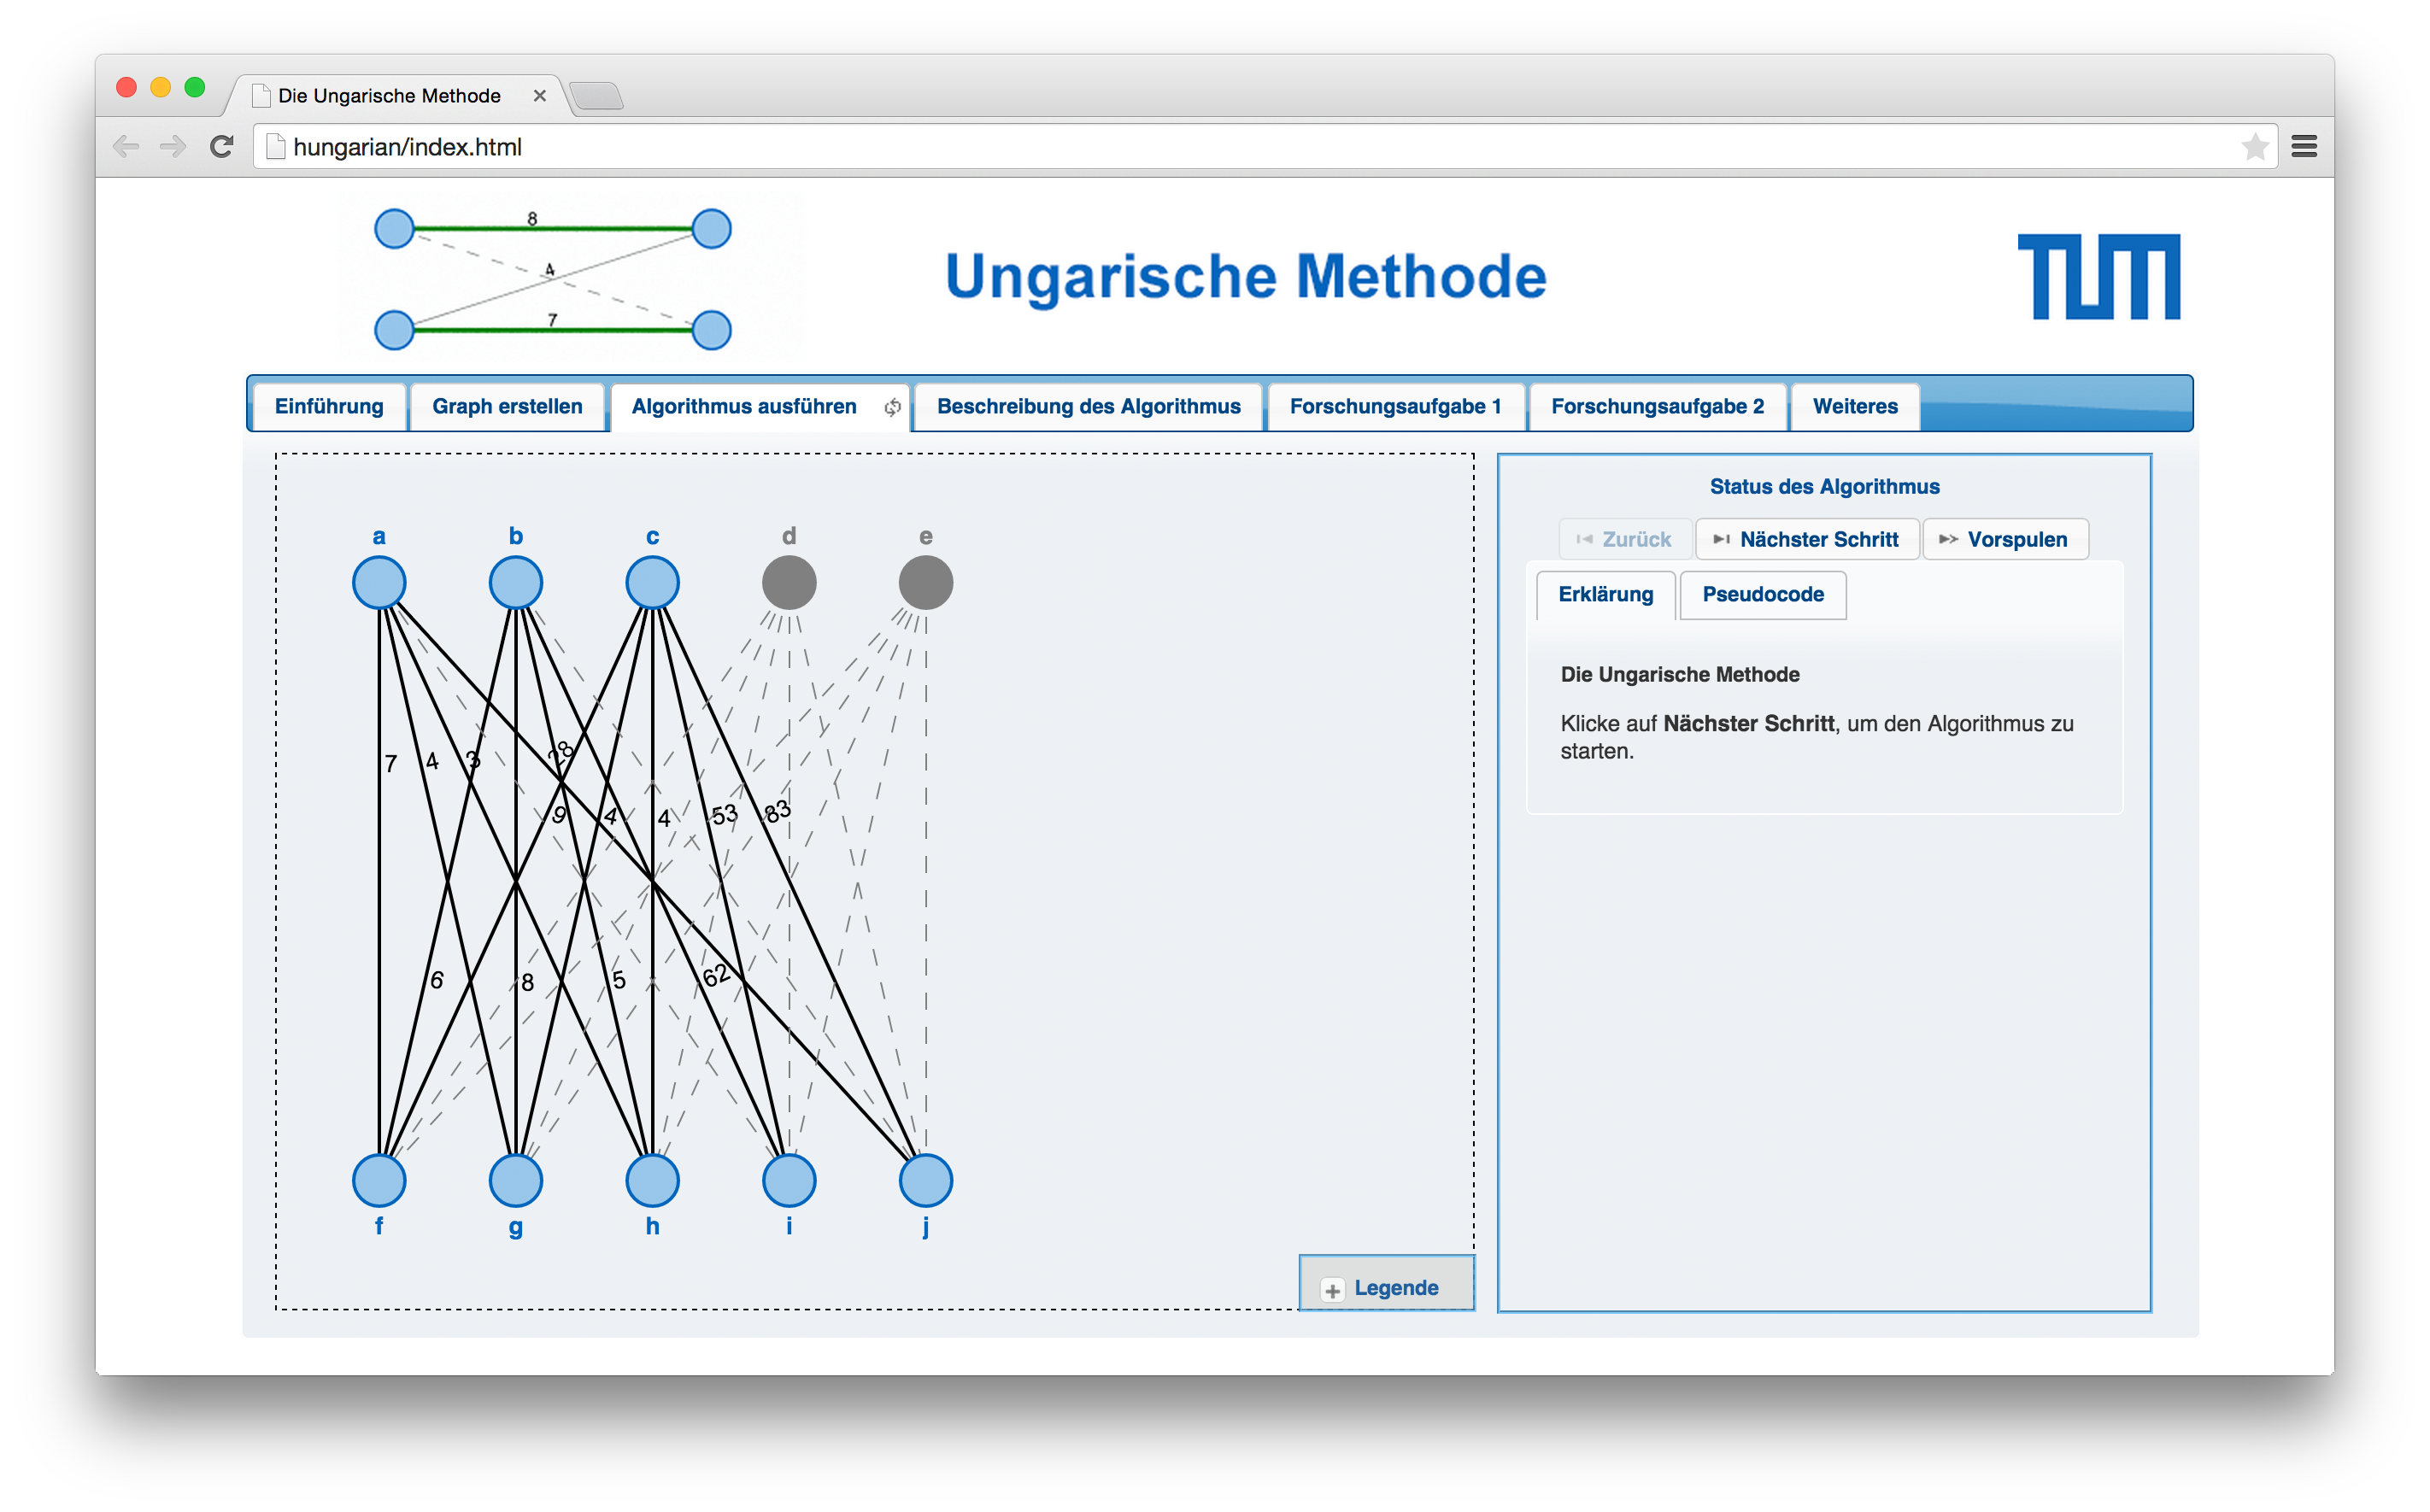
\includegraphics[width=\textwidth]{figures/hungarian-complete}
	\caption[Ungarische Methode]{Der Graph wird mit fehlenden Knoten und Kanten erweitert}\label{fig:hungarian-complete}
\end{figure}

\section{Multigraphen}%Ruslan
%Motivation
In bisherigen auf dem Framework basierenden Algorithmen war es nicht möglich Multikanten zu erstellen, was aber für die Algorithmen nicht notwendig war. Es war möglich maximal zwei Kanten zwischen zwei Knoten einzufügen. 
In dem Chinese-Postman-Algorithmus werden während der Ausführung Kanten in den Graphen eingefügt. Deshalb muss das Graphenmodell für den Chinese-Postman-Algorithmus mit Multikanten darstellen können. Die Abbildung \ref{fig:multigraph} zeigt einen Graphen mit Multikanten.
%Beispiel
\begin{figure}[h!]
	\centering
	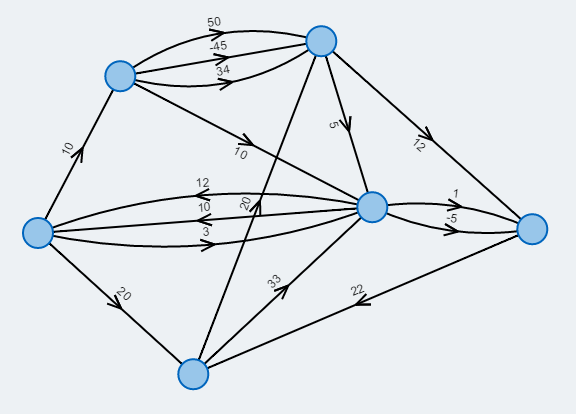
\includegraphics[width=\textwidth]{figures/multigraph}
	\caption[Multigraph]{Multikanten im Graphen}\label{fig:multigraph}
\end{figure}

\section{Zufällig generierte Fragen (Mark)}
In bisherigen auf diesem Framework basierenden Projekten war die Varianz der Fragen in den Forschungsaufgaben problematisch. Die Forschungsaufgaben behandelten meistens statische Fragen an vorher festgelegten Stellen zu vorgegebenen Graphen. Daraus resultierend bietet sich dem Nutzer ein wenig abwechslungsreiches Erlebnis und die Motivation, eine Forschungsaufgabe mehrfach zu bearbeiten, ist nicht gegeben.

In unserer Implementierung verfolgen wir daher einen anderen Ansatz. Die Forschungsaufgaben sind grundsätzlich so aufgebaut, dass sie die gleiche Struktur und den gleichen Quellcode wie die reguläre Ausführung des Algorithmus benutzen. Das schließt auch den vom Nutzer selbst gewählten Graph aus dem \enquote{Graph erstellen} Tab mit ein. Statt statischen Fragen definiert der Entwickler eine Menge von Fragetypen. Vor jedem Schritt des Algorithmus wird dann anhand einer Wahrscheinlichkeitsmatrix bestimmt, ob zu dem folgenden Schritt eine Frage gestellt wird und wenn ja, welcher Fragetyp gewählt werden soll. Außerdem sollen wenn möglich die Inhalte der generierten Fragen eines Fragetyps variieren. So werden beispielsweise die Knoten, zu denen ein Wert bestimmt werden soll, zufällig gewählt (vgl. Abbildung~\ref{fig:random-question}).

Mit dieser Implementierung gelingt es, dass in jeder Bearbeitung einer Forschungsaufgabe unterschiedliche Kombinationen von Fragen gestellt werden. Zusätzlich kann der Nutzer durch selbst erstelle Graphen auch Spezialfälle testen.

\begin{figure}[h!]
	\centering
	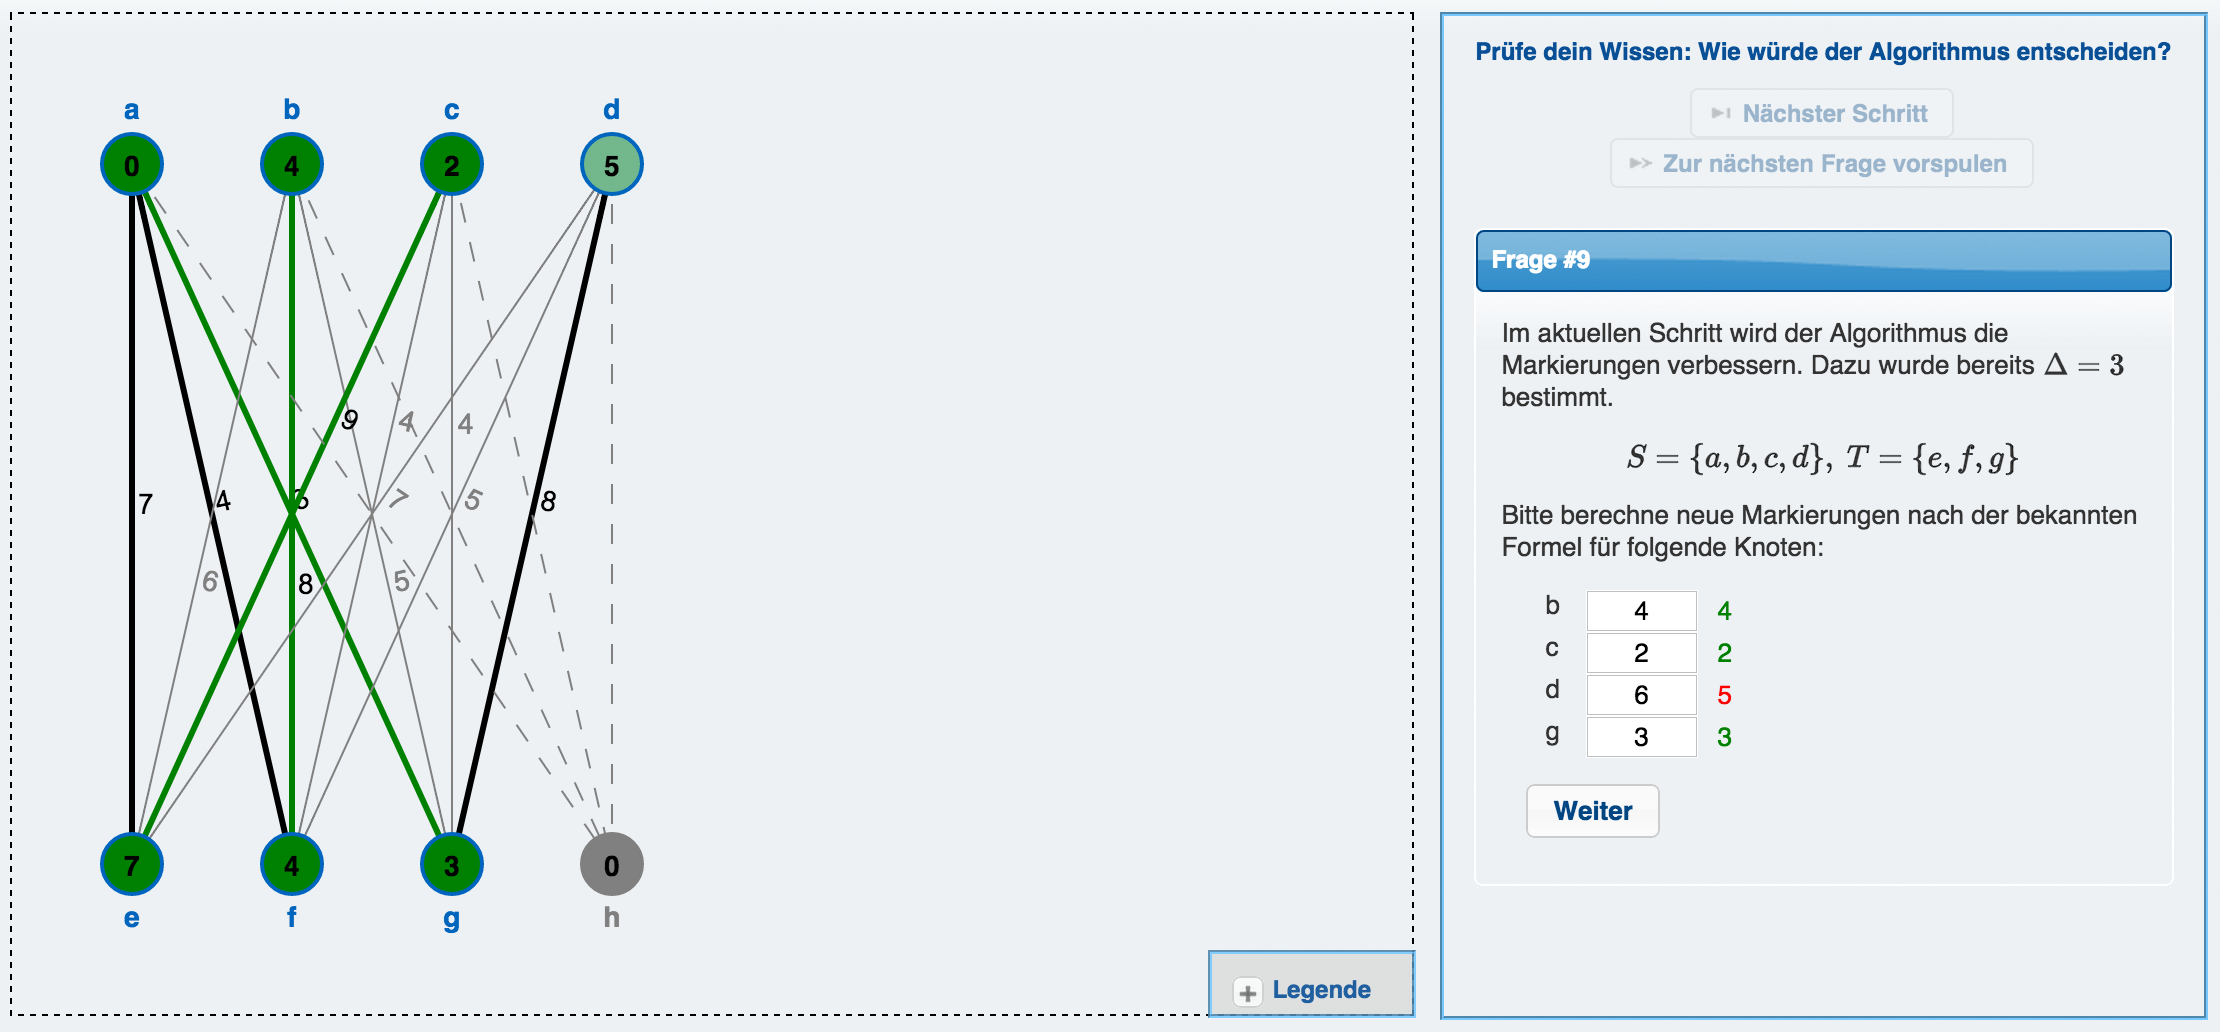
\includegraphics[width=\textwidth]{figures/random_question}
	\caption[Zufällig generierte Frage]{Beispiel für eine zufällig generierte Frage}\label{fig:random-question}
\end{figure}

\subsection*{Implementierung}
In der Funktion \texttt{this.nextStepChoice} wird vor der Auswahl des nächsten Schritts des Algorithmus mittels der Funktion \texttt{this.askQuestion} bestimmt, ob und welche Frage gestellt werden soll. Für jeden Fragetyp exisiert eine separate Funktion (bspw. \texttt{this.generateNextStepQuestion}), die auf den aktuellen Graph zugreift und eine Frage mit zufälligen Elementen generiert und in das DOM Element \texttt{\#tf1\_div\_questionModal} schreibt. Die gegebene Antwort wird durch Aufruf der Funktion \texttt{this.saveAnswer} gespeichert und mit der richtigen Lösung verglichen. Am Ende der Forschungsaufgabe kann mittels \texttt{this.showQuestionResults} eine Übersicht angezeigt werden, die zeigt, wieviele Fragen richtig beantwortet wurden. Weitere Informationen sind der Inline-Dokumentation zu entnehmen.

\section{Gemeinsam genutzte Dateien (Mark)}
Im Rahmen dieses interdisziplinären Projekts wurden Webapplikationen für insgesamt fünf Algorithmen entwickelt. Jede Applikation liegt in einem von den anderen Algorithmen unabhängigen Projektordner, der jeweils auch das Graph Framework aus früheren Projekten enthält. Daher lagen im gesamten Repository viele Dateien mehrfach vor. Dies war insofern problematisch, da Änderungen, die alle Anwendungen betreffen in mehreren Dateien vorgenommen werden mussten.

Unser Ziel war es daher, gemeinsam genutzte Dateien auszulagern. Wir beschränken uns hier auf Dateien, welche das Layout und Design der Anwendungen definieren sowie universelle Programmbibliotheken (bspw. MathJAX). Diese Beschränkung ist notwendig, um die Flexibilität im Entwicklungsprozess zu gewährleisten. Es existieren weitere Dateien, die sich zum aktuellen Zeitpunkt anwendungsübergreifend nicht signifikant unterscheiden. Diese sind allerdings algorithmenspezifisch und könnten in zukünftigen Entwicklungsphasen weiter verändert werden.

Zur Auslagerung legten wir zunächst einen \texttt{library} Ordner an. Das Finden von Dateiduplikaten übernimmt ein Python Skript (vgl. \texttt{deduplicate.py}), welches mittels der \texttt{difflib} Bibliothek alle Dateien in den Projektordnern paarweise miteinander vergleicht und einen Ähnlichkeitsquotienten bestimmt. Das Skript zeigt dann alle Dateien, die einen festgelegten Änhlichkeitsgrenzwert überschreiten an (vgl. Abbildungen \ref{fig:shared-files-1} und \ref{fig:shared-files-2}). Anhand des Quotienten lässt sich ablesen, ob Dateien im Gesamten oder in Teilen ausgelagert werden können. Das Verschieben in den \texttt{library} Ordner und die Anpassung der Pfade in den Anwendungen erfolgt dann manuell.

\begin{figure}[h!]
\noindent\texttt{chinese-postman/img/TUMLogo.png \\
-> 100.00\% identical to floyd-warshall/img/TUMLogo.png \\
-> 100.00\% identical to hierholzer/img/TUMLogo.png \\
-> 100.00\% identical to hopcroft-karp/img/TUMLogo.png \\
-> 100.00\% identical to hungarian/img/TUMLogo.png
}
\caption[Gemeinsame Dateien, Beispiel 1]{Vollständige Übereinstimmung bei der Datei \texttt{TUMLogo.png}}\label{fig:shared-files-1}
\end{figure}

\begin{figure}[h!]
\noindent\texttt{chinese-postman/js/siteAnimation.js \\
-> 67.01\% identical to hierholzer/js/siteAnimation.js \\
-> 91.49\% identical to hopcroft-karp/js/siteAnimation.js \\
-> 71.13\% identical to hungarian/js/siteAnimation.js
}
\caption[Gemeinsame Dateien, Beispiel 2]{Mäßige Übereinstimmungen bei der Datei \texttt{siteAnimation.js}}\label{fig:shared-files-2}
\end{figure}

Für zukünftige Projekte können die Parameter des Skripts angepasst werden. Weitere Informationen hierzu sind der Inline-Dokumentation zu entnehmen.

\chapter{Zusammenfassung}
%Zusammenfass.
Das interdisziplinäre Projekt beschäftigt sich mit der anschaulichen Darstellung von weiterführenden Graphalgorithmen. Vorgestellt werden folgende Probleme: All-Pairs Shortest Path Problem, Matchingprobleme in bipartiten Graphen, das Eulertour Problem und das Chinese-Postman-Problem. 
Die Problemstellungen werden mit einfachen Worten erklärt und die verwendeten Lösungsverfahren interaktiv veranschaulicht. Die Darstellung der Algorithmen erfolgt in Form mehrerer Web-Applikationen, die auf ein gemeinsames Framework aufbauen, welches bereits bei früheren Projekten zum Einsatz kam. In den Applikationen wird der Benutzer zunächst an die jeweilige Problemstellung herangeführt. Anschließend erhält er die Möglichkeit die Algorithmen auf selbst erstellten Graphen schrittweise ausführen zu lassen. Außerdem werden speziellen Eigenschaften der Algorithmen in gesonderten Forschungsaufgaben behandelt. 

%Neues
Im Rahmen des Projekts wurden mehrere Änderungen und Weiterentwicklungen an dem Framework durchgeführt. Für Matchingprobleme auf bipartiten Graphen wurde ein bipartites Graphenmodell und die zugehörige Visualisierung entwickelt. Für den Chinese-Postman-Algorithmus wurde ein Graphenmodell entwickelt, das Multikanten unterstützt. 
Die MathJax-Bibliothek ermöglicht in der Beschreibung der Algorithmen mathematische Formeln einzusetzen. Dadurch können wichtige Aspekte der Algorithmen als mathematische Formeln dargestellt werden, sodass das Grundverständnis der Algorithmen dem Benutzer besser vermittelt werden kann.
Um die Motivation, eine Forschungsaufgabe mehrfach zu bearbeiten, zu erhöhen, wurden dynamische Fragen erstellt. Die Anzahl der Fragen hängt von dem Graphen ab und der Fragetyp wird während der Abarbeitung zufällig ausgewählt. Da das vorliegende interdisziplinäre Projekt eine Gruppenarbeit darstellt, war es möglich identische und gemeinsam genutzte Dateien auszulagern. Dadurch existieren sie nur einmal, was eventuelle Änderungen an dem Projekt vereinfacht.
